
%%%%%%%%%%%%%%%%%%%%%%%%%%%%%%%%%%%%%%%%%%%%%%%%%%%%%%%
%%	Code Snippet										%%
%%	This template is used for a report with codes.	%%
%%%%%%%%%%%%%%%%%%%%%%%%%%%%%%%%%%%%%%%%%%%%%%%%%%%%%%%

\documentclass[a4paper,12pt]{article}


%%%%%%%%%%%%%%%%%%%%%% Start of packages %%%%%%%%%%%%%%%%%%%%%%%%%
\usepackage[english]{babel}
\usepackage[latin1]{inputenc}
\usepackage{listings} % Required for inserting code snippets
\usepackage[usenames,dvipsnames]{color} % Required for specifying custom colors and referring to colors by name

%	Define Paper's structure
\usepackage[top=2cm,bottom=3.5cm]{geometry}

%	Enable to insert/edit an image into the report
\usepackage{graphicx}
\usepackage{wrapfig}
\usepackage{epstopdf}
\usepackage{color}

%	Common Tools
%\usepackage[]{hyperref}		% Enable to use hyperlink in PDF
\usepackage{enumerate}		% Enable to enumerate items
\usepackage{indentfirst}		% force to indent the firsr line of all paragraphes
\usepackage{textcomp}		% Insert special characters
\usepackage{cite}			% Use special characters
\usepackage{amsmath}
\usepackage{amssymb}
\usepackage{amsthm}
\usepackage{amsfonts}
\usepackage{tabularx}
\usepackage{comment}
\usepackage{multirow}
\usepackage{tabularx}
\usepackage{booktabs}
\usepackage{multicol}
\usepackage{xcolor}
\usepackage{caption}
\usepackage{subcaption}
\usepackage{scrextend}
\usepackage{bbm}

\usepackage{mathtools}
\DeclarePairedDelimiter\ceil{\lceil}{\rceil}
\DeclarePairedDelimiter\floor{\lfloor}{\rfloor}

% plot UML
\usepackage[simplified]{pgf-umlcd}


\newenvironment{changemargin}[2]{%
\begin{list}{}{%
	\setlength{\topsep}{0pt}%
	\setlength{\leftmargin}{#1}%
	\setlength{\rightmargin}{#2}%
	\setlength{\listparindent}{\parindent}%
	\setlength{\itemindent}{\parindent}%
	\setlength{\parsep}{\parskip}%
}%
\item[]}{\end{list}}


%%%%%%%%%%%%%%%%%%%%%%% End of packages %%%%%%%%%%%%%%%%%%%%%%%

\setlength{\tabcolsep}{12pt}
\deffootnote{0em}{1.6em}{\thefootnotemark.\enskip}

% Define different highlight color used in code
\definecolor{DarkGreen}{rgb}{0.0,0.4,0.0}
\definecolor{highlight}{RGB}{255,251,204}

\numberwithin{equation}{section}
\DeclareMathOperator*{\argmin}{arg\,min}
\DeclareMathOperator*{\argmax}{arg\,max}
\newcommand{\ra}[1]{\renewcommand{\arraystretch}{#1}}

% Define the style of code
\lstdefinestyle{Style1}{
	language=python, % Detects keywords, comments, strings, functions, etc for the language specified
	backgroundcolor=\color{highlight}, % Set the background color for the snippet - useful for highlighting
	basicstyle=\footnotesize\ttfamily, % The default font size and style of the code
	breakatwhitespace=false, % If true, only allows line breaks at white space
	breaklines=true, % Automatic line breaking (prevents code from protruding outside the box)
	captionpos=b, % Sets the caption position: b for bottom; t for top
	commentstyle=\usefont{T1}{pcr}{m}{sl}\color{DarkGreen}, % Style of comments within the code - dark green courier font
	deletekeywords={}, % If you want to delete any keywords from the current language separate them by commas
	%escapeinside={\%}, % This allows you to escape to LaTeX using the character in the bracket
	firstnumber=1, % Line numbers begin at line 1
	frame=single, % Frame around the code box, value can be: none, leftline, topline, bottomline, lines, single, shadowbox
	frameround=tttt, % Rounds the corners of the frame for the top left, top right, bottom left and bottom right positions
	keywordstyle=\color{Blue}\bf, % Functions are bold and blue
	morekeywords={}, % Add any functions no included by default here separated by commas
	numbers=left, % Location of line numbers, can take the values of: none, left, right
	numbersep=10pt, % Distance of line numbers from the code box
	numberstyle=\tiny\color{Gray}, % Style used for line numbers
	rulecolor=\color{black}, % Frame border color
	showstringspaces=false, % Don't put marks in string spaces
	showtabs=false, % Display tabs in the code as lines
	stepnumber=5, % The step distance between line numbers, i.e. how often will lines be numbered
	stringstyle=\color{Purple}, % Strings are purple
	tabsize=2, % Number of spaces per tab in the code
}

% Create a command to insert a snippet with the style above anywhere in the document
\newcommand{\insertcode}[2]{\begin{itemize}\item[]\lstinputlisting[caption=#2,label=#1,style=Style1]{#1}\end{itemize}} % The first argument is the script location/filename and the second is a caption for the listing


%%%%%%%%%%%%%%% Start of front cover's page %%%%%%%%%%%%%%%%%%%

%	Set title
\title{Project APC 524}

%	Set authors
\author{Guanhua He (Molbio), Ping Wu (Molbio), Zongjun Tan (ORFE)}

%%%%%%%%%%%%%%% End of front cover's page %%%%%%%%%%%%%%%%%%%%%


%%%%%%%%%%%%%%% Begin of the document %%%%%%%%%%%%%%%%%%%
 
\begin{document}
 \maketitle
 %\tableofcontents
	
%	We consider dimension 1 situation, namely $x \in \mathbb{R}$. Let $\mu \in \mathcal{P}(\mathbb{R})$ be a distribution in $\mathbb{R}$.  \\
	%%%%%%%%%%%%%%%%%%%% Begin of the Section 1 %%%%%%%%%%%%%%%%%%%%%%%%%%
	
	\section{Task description}
	
This project is about to improve some image analyzing codes and their performance related to a study on drosophila embryo conducted by one of our group
members Ping Wu. She uses some fluorescent antibodies to stain for endogenous proteins to get spatial gene expression profiles at certain stage of embryonic development. Then, she will infer how the perturbation exerted on the embryos affect the transcription network and downstream gene expression base on the profile. Before making any biological analysis, she requires to extract fluorescent intensities from each cell along the whole embryo,
Given the above background information, we would like to achieve two objectives in this project. The first one is to create an interface adapted to the existing
codes in order to facilitate the future development in her own research. The second objective tends to improve automation. The initial image processing is still done manually currently, which is time consuming. The initial step requires recognition the morphology of the embryo and distinguish head and tail, dorsal and ventral side, and then rotate and center the object. Some noise removal steps are also required. If we have spare time, we could adapt this code to a series of time lapse images, with cell tracking function and parallel computing function for large scale image processing.


%%%%%%%%%%%%%%
	
	\section{Organization}

	\subsection{Goal}[detail description will be completed by Ping]
	
	A group of drosophila embryos that lie on a plane have been photographed in order to keep track of the development of 4 genes' spatial expression profiles (say ``gene" for short in the following). At a special given time, we are provided with a collection of images corresponded to different sample embryos as well as their gene profiles. Each sample embryo has 4 different gene profiles.
	
	{\color{red} Question: please describe how many gene profiles do we have? different gene expression profile due to how many different situations? }
	
	Our objective is the following: 
	\begin{enumerate}
		\item Rotate the sample embryo in an image so that the line from head to tail of that embryo is level.
		\item Detect meaningful area of/inside a sample embryo image to extract the luminosity information of gene expression.
		\item [Optimal:] Create a mask from a particular gene expression of a sample embryo, and then apply this mask to other gene expressions of the same embryo in order to detect luminosity information of other genes.
	\end{enumerate} 
	
	\subsection{Design pattern}
	The codes will be written in Python. 
	
	\subsubsection{detail description}
	
	\begin{tabular}{ l  l| l}	
		\multicolumn{3}{c}{Embryo}\\
		\hline
		attribute &  type & Description\\
		\hline \hline
		gene\_name & String & name of the gene\\
		spatial\_loc\_rgb & $2d\times3$ array & rgb image of the spatial gene expression\\
		&& in an embryo\\
		spatial\_loc & 2d array & gray scale image of \textit{spatial\_loc\_rgb}\\
		\hline\hline
		method & return type & description\\
		\hline
		read\_from\_filename & $2d \times 3$ array & read an rgb image from a filename,\\
		&& store it in \textit{spatial\_loc} \\
		read\_from\_array & $2d \times 3$ array & read an rgb image from a 2d array,\\
		&& store it in  \textit{spatial\_loc}\\
		rgb2gray &  2d array & convert to gray scale image\\
		\hline
	\end{tabular}
	
	
	\subsubsection{Hierarchy between classes}
	
	\begin{minipage}[c]{1.5\textwidth}
	\begin{changemargin}{-3cm}{-3cm}

	\begin{small}
	
	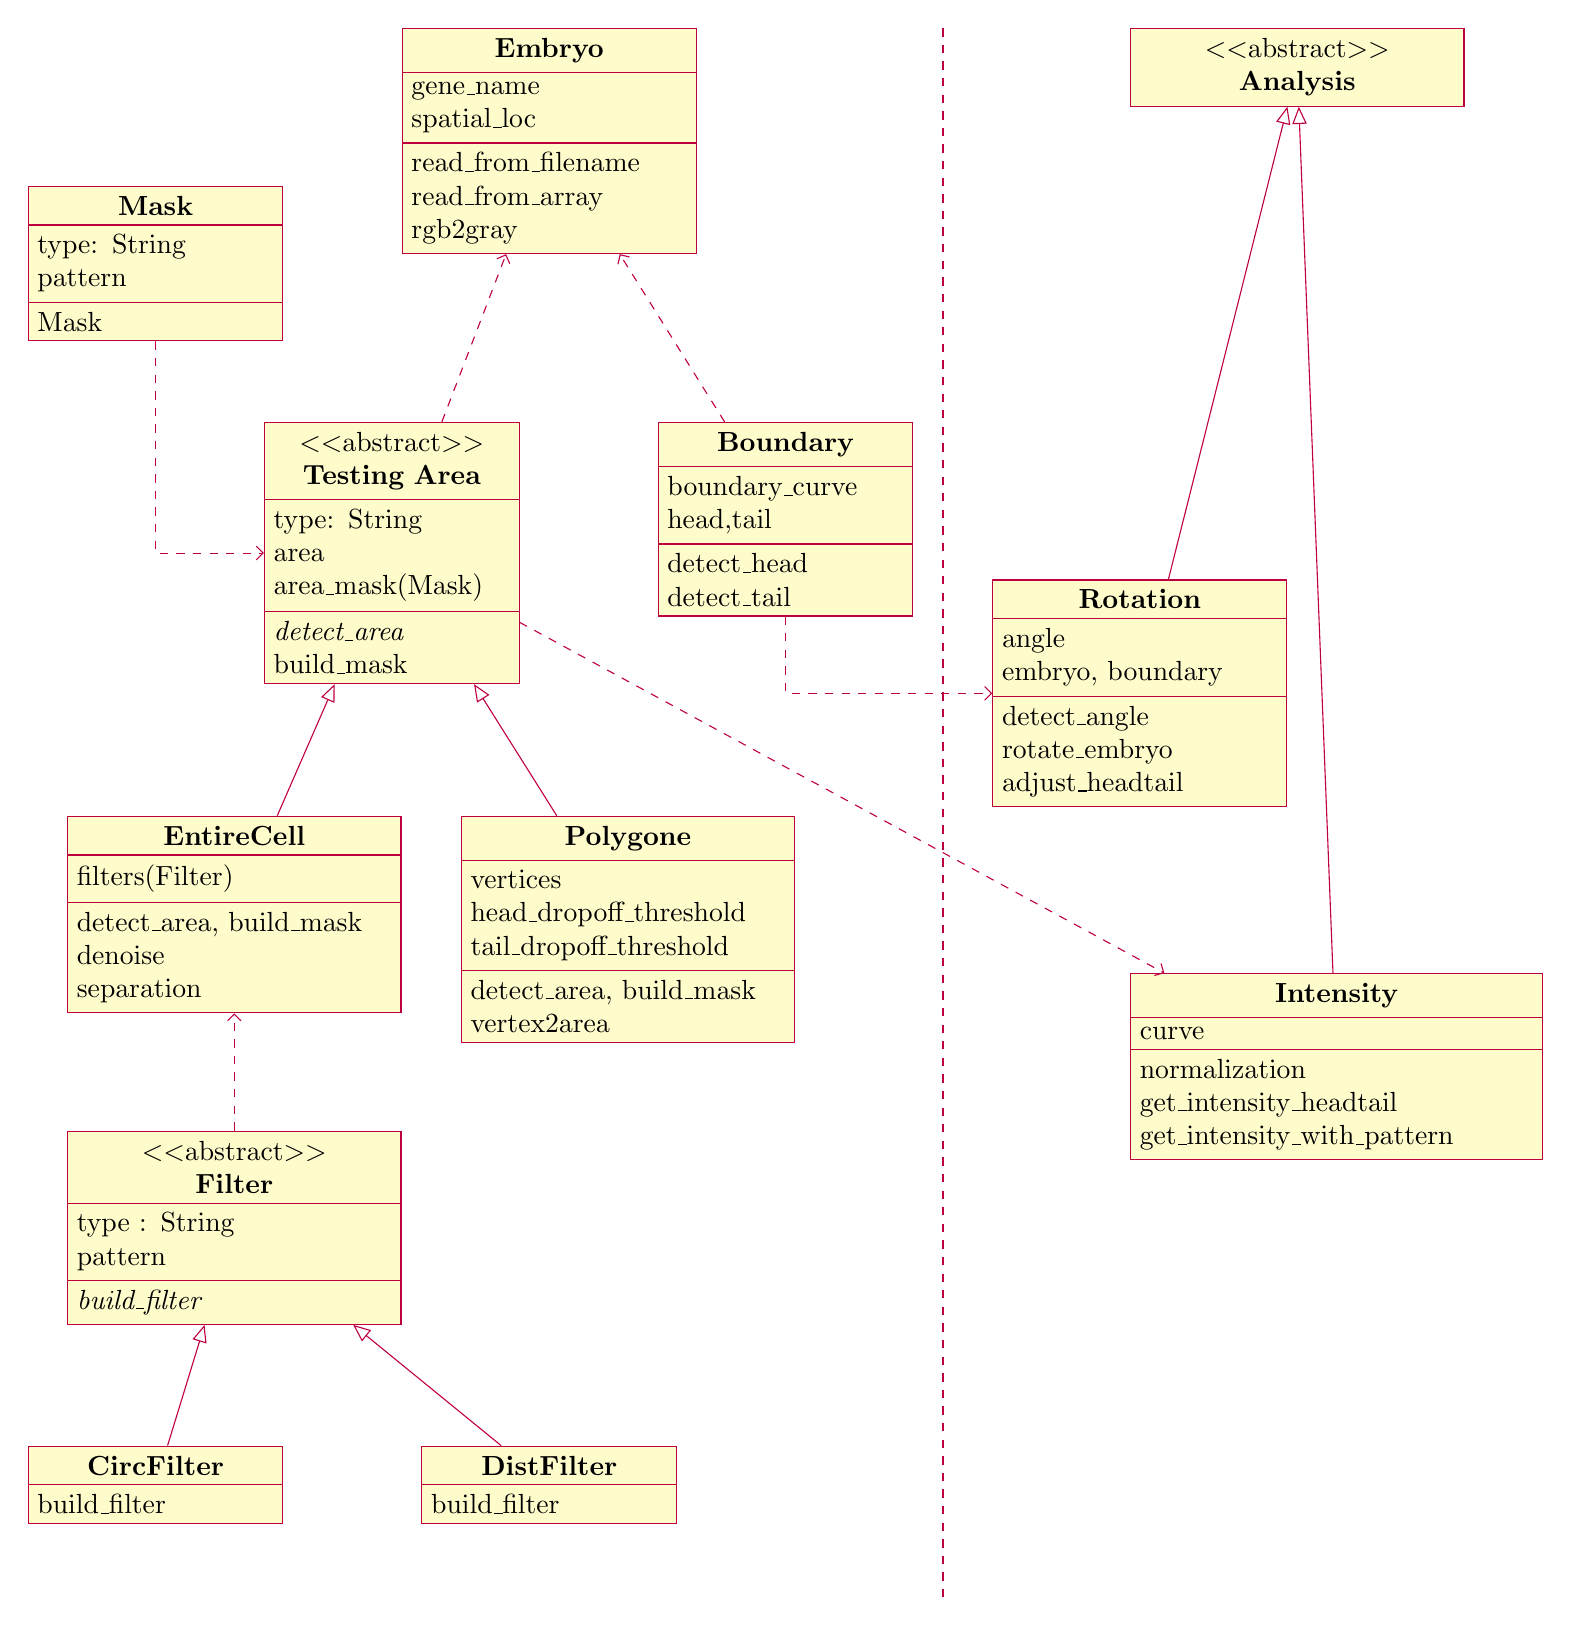
\begin{tikzpicture}%[show background grid]
	
		\begin{class}[text width=3.5cm]{Embryo}{-3,2}
			\attribute{gene\_name}
			\attribute{spatial\_loc}
			
			\operation{read\_from\_filename}
			\operation{read\_from\_array}
			\operation{rgb2gray}
		\end{class}
		
		\begin{class}[text width=3cm]{Boundary}{0,-3}
			\attribute{boundary\_curve}
			\attribute{head,tail}
			
			\operation{detect\_head}
			\operation{detect\_tail}
		\end{class}
		
		
		%% Testing area
		\begin{abstractclass}[text width =3cm]{Testing Area}{-5,-3}
			\attribute{type: String}
			\attribute{area}
			\attribute{area\_mask(Mask)}
			% abstract method
			\operation[0]{detect\_area}
			\operation{build\_mask}
		\end{abstractclass}
		
		
		\begin{class}[text width = 4cm]{Polygone}{-2,-8}
		\inherit{Testing Area}
			\attribute{vertices}
			\attribute{head\_dropoff\_threshold}
			\attribute{tail\_dropoff\_threshold}
			
			\operation{detect\_area, build\_mask}
			\operation{vertex2area}
		\end{class}
		
		\begin{class}[text width= 4cm]{EntireCell}{-7,-8}
		\inherit{Testing Area}
			\attribute{filters(Filter)}
			
			\operation{detect\_area, build\_mask}
			\operation{denoise}
			\operation{separation}
		\end{class}
		
		
		% Mask
		\begin{class}[text width=3cm]{Mask}{-8,0}
			\attribute{type: String}
			\attribute{pattern}
		
			\operation{Mask}
		\end{class}
		
		
		%% Filter class
		\begin{abstractclass}[text width=4cm]{Filter}{-7,-12}
		\attribute{type : String}
		\attribute{pattern}
		
		\operation[0]{build\_filter}
		\end{abstractclass}
		
		\begin{class}[text width=3cm]{CircFilter}{-8, -16}
		\inherit{Filter}
		\operation{build\_filter}
		\end{class}
		
		\begin{class}[text width=3cm]{DistFilter}{-3,-16}
		\inherit{Filter}
		\operation{build\_filter}
		\end{class}
		
		
		
		%% Analysis
		\begin{abstractclass}[text width =4cm]{Analysis}{6.5,2}
		\end{abstractclass}
		
		\begin{class}[text width=3.5cm]{Rotation}{4.5,-5}
		\inherit{Analysis}
			\attribute{angle}
			\attribute{embryo, boundary}
			
			\operation{detect\_angle}
			\operation{rotate\_embryo}
			\operation{adjust\_headtail}
		\end{class}
				
				
		\begin{class}[text width=5cm]{Intensity}{7, -10}
		\inherit{Analysis}
			\attribute{curve}
		
			\operation{normalization}
			\operation{get\_intensity\_headtail}
			\operation{get\_intensity\_with\_pattern}
		\end{class}
		
		
		%\aggregation{Embryo}{external}{1}{Boundary}
		%\aggregation{Embryo}{area}{1}{Testing Area}
		\draw[umlcd style dashed line , ->](Testing Area)--node[above,sloped,black]{}(Embryo);
		\draw[umlcd style dashed line , ->](Boundary)--node[above,sloped,black]{}(Embryo);
		
		\draw[umlcd style dashed line , ->](Boundary)|-node[above,sloped,black]{}(Rotation);
		
		\draw[umlcd style dashed line , ->](Mask)|-node[above,sloped,black]{}(Testing Area);
		
		\draw[umlcd style dashed line , ->](Filter)--node[above,sloped,black]{}(EntireCell);
		
		\draw[umlcd style dashed line , ->](Testing Area)--node[below,sloped,black]{}(Intensity);
		
		\draw[umlcd style dashed line] (2,2)--(2,-18);
		
	\end{tikzpicture}
	
	\end{small}
	\end{changemargin}
	\end{minipage}
	
%%%%%%%%%%%%%%%%%%%%%%
	\newpage
	\section{Schedule}
	In total 8 weeks.
	
	\begin{itemize}
		\item Nov 18 (Sun) -- Nov 24 (Sat) (Thanksgiving week):  
		
		Discuss the project with Gabe. Question: what should be included in the prototype? To which extend should we do parallelization? How to represent profiling checking?  
		
		Read reference papers of Ping's project.
		
		Understand properly the existence code structure. (potentially 1 extra meeting) 
		Clarification of all relationships between existing functions and their input/output. 
		
		List one or two potential requires in the future development.(Ping)
		
		First version of the prototype. (Graphical + coding)
		
		
		\item Nov 25 (Sun) -- Dec 1 (Sat) : 
		  
		Second version of the prototype. 
		
		Familiar with parallel programming.
		
		Familiar with location detection techniques in the existing codes.(To be done) 
		
		\item Dec 2 (Sun) -- Dec 8 (Sat): 
		
		prepare for presenting the prototype in course. (third version)
		
		alpha version of parallelization.
		
		\item Dec 9 (Sat) -- Dec 15 (Sat):
		
		Improve parallelization. 
		
		\item Dec 16 (Sun) -- Dec 22 (Sat) [Winter Break]:
		\item Dec 23 (Sun) -- Dec 29 (Sat) [Winter Break]:
		\item Dec 30 (Sun) -- Jan 5  (Sat) [Winter Break]:
		\item Jan 6 (Sun) -- Jan 12 (Sat):
		
		
		
		 
		
	\end{itemize}
	
	%%%%%%%%%%%%%%%%%%%%%%%%%%%%%%%%%%%%%%%%%%%%%%%%%%%%%%%%%%%

	%%%%%%%%%%%%%%%%%%%%%%%%%%%%%%%

	%%%%%%%%%%%%%%%%%%%%%%%%%%%%%%
	%\newpage
	\bibliographystyle{plain}
	\bibliography{}{}
	

\end{document}
